\usepackage{pgfplots}

\usepgfplotslibrary{patchplots}
\pgfplotsset{compat=1.6}

\begin{document}
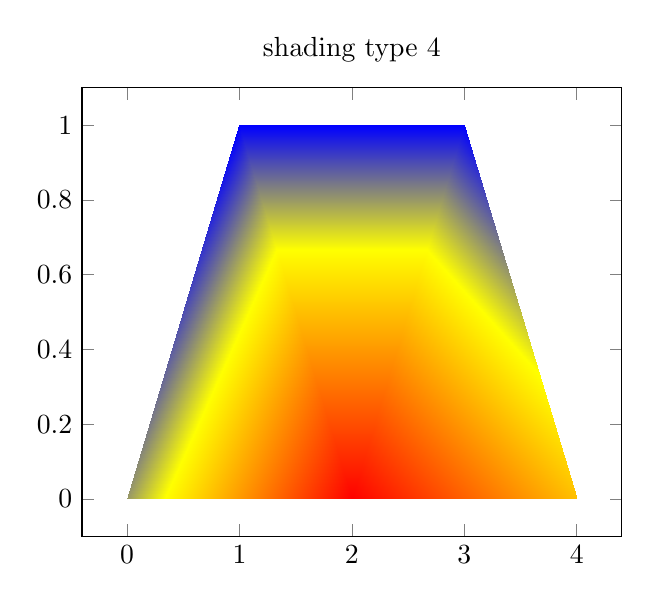
\begin{tikzpicture}
    \begin{axis}[title=shading type 4]
    \addplot[patch,shader=interp]
    table[point meta=\thisrow{c}] {
        x y c
        0 0 0.2
        1 1 0
        2 0 1
        1 1 0
        2 0 1
        3 1 0
        2 0 1
        3 1 0
        4 0 0.5
    };
    \end{axis}
\end{tikzpicture}


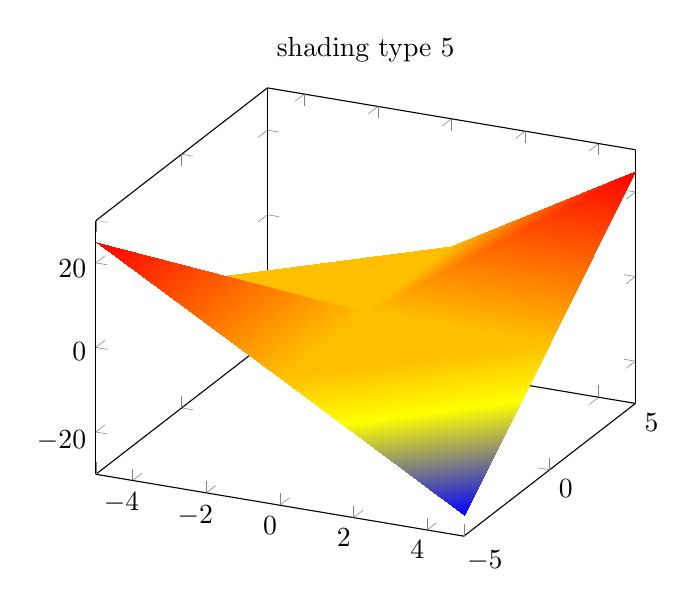
\begin{tikzpicture}
	\begin{axis}[title=shading type 5]
	\addplot3[surf,shader=interp,samples=3] {x*y};	
	\end{axis}
\end{tikzpicture}

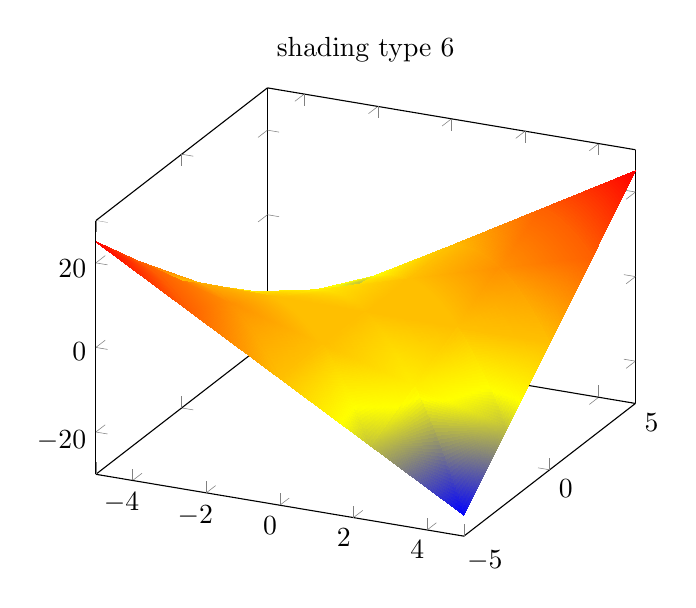
\begin{tikzpicture}
	\begin{axis}[title=shading type 6]
	\addplot3[
		surf,
		patch type=triangle quadr,
		patch type sampling, 
		samples=5,
		shader=interp] {x*y};	
	\end{axis}
\end{tikzpicture}

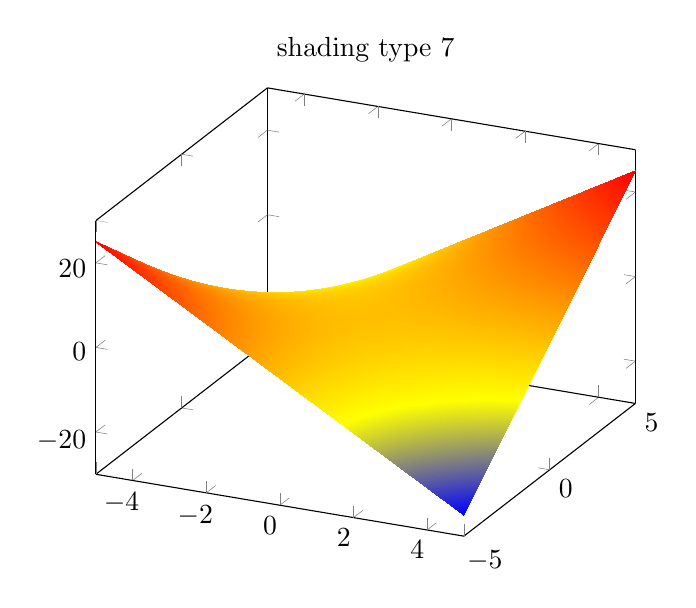
\begin{tikzpicture}
	\begin{axis}[title=shading type 7]
	\addplot3[
		surf,
		patch type=bicubic,
		patch type sampling, 
		samples=5,
		shader=interp] {x*y};	
	\end{axis}
\end{tikzpicture}

\end{document}
